% Source taken from https://arxiv.org/abs/2203.05570
% Compile with:
% latexmk -lualatex neos-pipeline.tex
% convert -density 300 neos-pipeline.pdf neos-pipeline.png
\RequirePackage{luatex85}
\documentclass[tikz, border=5pt]{standalone}

\begin{document}

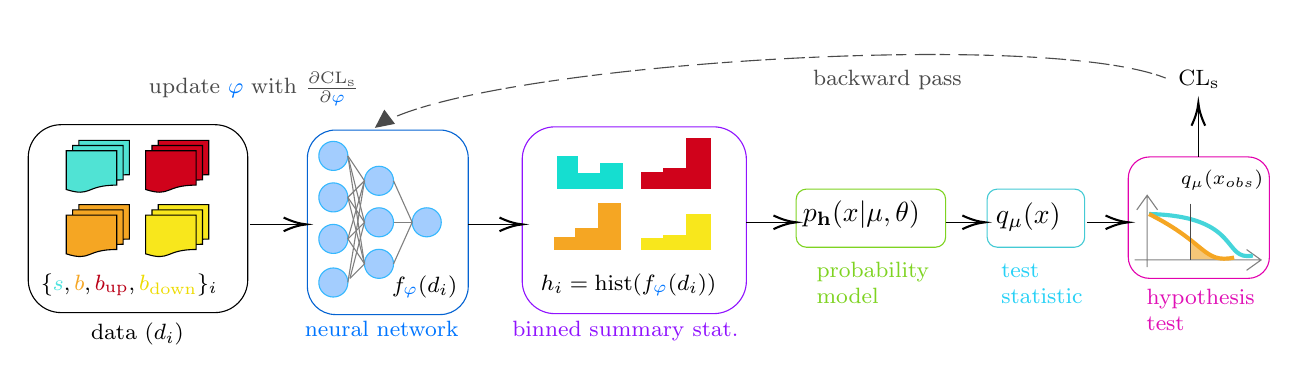
\begin{tikzpicture}[x=0.75pt,y=0.75pt,yscale=-1,xscale=1]
%uncomment if require: \path (0,162); %set diagram left start at 0, and has height of 162

%Shape: Right Triangle [id:dp362300353514037]
\draw  [draw opacity=0][fill={rgb, 255:red, 246; green, 199; blue, 120 }  ,fill opacity=1 ] (562,106) -- (576.67,114) -- (562,114) -- cycle ;
%Shape: Axis 2D [id:dp12893196021028852]
\draw [color={rgb, 255:red, 128; green, 128; blue, 128 }  ,draw opacity=1 ] (535,114.13) -- (596,114.13)(541.1,83) -- (541.1,117.59) (589,109.13) -- (596,114.13) -- (589,119.13) (536.1,90) -- (541.1,83) -- (546.1,90)  ;
%Curve Lines [id:da5288049156007071]
\draw [color={rgb, 255:red, 69; green, 213; blue, 218 }  ,draw opacity=1 ][line width=1.5]    (542,92) .. controls (587,93) and (577,115) .. (592,112) ;
%Curve Lines [id:da8563594209924821]
\draw [color={rgb, 255:red, 245; green, 166; blue, 35 }  ,draw opacity=1 ][line width=1.5]    (542,92) .. controls (570,106) and (568,116) .. (583,113) ;

%Shape: Rectangle [id:dp06559015102114318]
\draw  [draw opacity=0][fill={rgb, 255:red, 21; green, 222; blue, 208 }  ,fill opacity=1 ] (256.84,64.01) -- (267.09,64.01) -- (267.09,79.96) -- (256.84,79.96) -- cycle ;
%Shape: Rectangle [id:dp05877121274370989]
\draw  [draw opacity=0][fill={rgb, 255:red, 21; green, 222; blue, 208 }  ,fill opacity=1 ] (267.09,72.38) -- (277.6,72.38) -- (277.6,79.96) -- (267.09,79.96) -- cycle ;
%Shape: Rectangle [id:dp5772101339046112]
\draw  [draw opacity=0][fill={rgb, 255:red, 21; green, 222; blue, 208 }  ,fill opacity=1 ] (277.6,67.2) -- (288.62,67.2) -- (288.62,79.96) -- (277.6,79.96) -- cycle ;

%Shape: Rectangle [id:dp5351184013195962]
\draw  [draw opacity=0][fill={rgb, 255:red, 245; green, 166; blue, 35 }  ,fill opacity=1 ] (255.08,103) -- (265.67,103) -- (265.67,109.5) -- (255.08,109.5) -- cycle ;
%Shape: Rectangle [id:dp3237986353533244]
\draw  [draw opacity=0][fill={rgb, 255:red, 245; green, 166; blue, 35 }  ,fill opacity=1 ] (265.61,98.86) -- (277.15,98.86) -- (277.15,109.5) -- (265.61,109.5) -- cycle ;
%Shape: Rectangle [id:dp028517110894384246]
\draw  [draw opacity=0][fill={rgb, 255:red, 245; green, 166; blue, 35 }  ,fill opacity=1 ] (276.41,86.46) -- (287.74,86.46) -- (287.74,109.5) -- (276.41,109.5) -- cycle ;
%Shape: Rectangle [id:dp7911777118441403]
\draw  [draw opacity=0][fill={rgb, 255:red, 208; green, 2; blue, 27 }  ,fill opacity=1 ] (297.45,71.69) -- (308.93,71.69) -- (308.93,79.96) -- (297.45,79.96) -- cycle ;
%Shape: Rectangle [id:dp7890938289430716]
\draw  [draw opacity=0][fill={rgb, 255:red, 208; green, 2; blue, 27 }  ,fill opacity=1 ] (307.99,69.91) -- (319.52,69.91) -- (319.52,79.96) -- (307.99,79.96) -- cycle ;
%Shape: Rectangle [id:dp7964104169097874]
\draw  [draw opacity=0][fill={rgb, 255:red, 208; green, 2; blue, 27 }  ,fill opacity=1 ] (318.78,55.14) -- (331,55.14) -- (331,79.96) -- (318.78,79.96) -- cycle ;

%Shape: Rectangle [id:dp41063858268086073]
\draw  [draw opacity=0][fill={rgb, 255:red, 248; green, 231; blue, 28 }  ,fill opacity=1 ] (297.45,103.59) -- (308.93,103.59) -- (308.93,109.5) -- (297.45,109.5) -- cycle ;
%Shape: Rectangle [id:dp4845140527035223]
\draw  [draw opacity=0][fill={rgb, 255:red, 248; green, 231; blue, 28 }  ,fill opacity=1 ] (307.99,102.33) -- (319.52,102.33) -- (319.52,109.5) -- (307.99,109.5) -- cycle ;
%Shape: Rectangle [id:dp16652300940730091]
\draw  [draw opacity=0][fill={rgb, 255:red, 248; green, 231; blue, 28 }  ,fill opacity=1 ] (318.78,91.77) -- (331,91.77) -- (331,109.5) -- (318.78,109.5) -- cycle ;

%Flowchart: Multidocument [id:dp01735535493895135]
\draw  [fill={rgb, 255:red, 80; green, 227; blue, 212 }  ,fill opacity=1 ] (26.4,56.5) -- (50.75,56.5) -- (50.75,73.06) .. controls (35.53,73.06) and (38.57,79.04) .. (26.4,75.17) -- cycle ; \draw  [fill={rgb, 255:red, 80; green, 227; blue, 212 }  ,fill opacity=1 ] (23.36,59.01) -- (47.7,59.01) -- (47.7,75.57) .. controls (32.49,75.57) and (35.53,81.55) .. (23.36,77.68) -- cycle ; \draw  [fill={rgb, 255:red, 80; green, 227; blue, 212 }  ,fill opacity=1 ] (20.32,61.52) -- (44.66,61.52) -- (44.66,78.08) .. controls (29.44,78.08) and (32.49,84.06) .. (20.32,80.19) -- cycle ;
%Flowchart: Multidocument [id:dp5524149748861067]
\draw  [fill={rgb, 255:red, 245; green, 166; blue, 35 }  ,fill opacity=1 ] (26.4,87.5) -- (50.75,87.5) -- (50.75,104.07) .. controls (35.53,104.07) and (38.57,110.04) .. (26.4,106.18) -- cycle ; \draw  [fill={rgb, 255:red, 245; green, 166; blue, 35 }  ,fill opacity=1 ] (23.36,90.01) -- (47.7,90.01) -- (47.7,106.58) .. controls (32.49,106.58) and (35.53,112.55) .. (23.36,108.69) -- cycle ; \draw  [fill={rgb, 255:red, 245; green, 166; blue, 35 }  ,fill opacity=1 ] (20.32,92.52) -- (44.66,92.52) -- (44.66,109.09) .. controls (29.44,109.09) and (32.49,115.06) .. (20.32,111.19) -- cycle ;
%Flowchart: Multidocument [id:dp05309909794201273]
\draw  [fill={rgb, 255:red, 208; green, 2; blue, 27 }  ,fill opacity=1 ] (64.66,56.5) -- (89,56.5) -- (89,73.06) .. controls (73.79,73.06) and (76.83,79.04) .. (64.66,75.17) -- cycle ; \draw  [fill={rgb, 255:red, 208; green, 2; blue, 27 }  ,fill opacity=1 ] (61.61,59.01) -- (85.96,59.01) -- (85.96,75.57) .. controls (70.74,75.57) and (73.79,81.55) .. (61.61,77.68) -- cycle ; \draw  [fill={rgb, 255:red, 208; green, 2; blue, 27 }  ,fill opacity=1 ] (58.57,61.52) -- (82.91,61.52) -- (82.91,78.08) .. controls (67.7,78.08) and (70.74,84.06) .. (58.57,80.19) -- cycle ;
%Flowchart: Multidocument [id:dp15006228098136898]
\draw  [fill={rgb, 255:red, 248; green, 231; blue, 28 }  ,fill opacity=1 ] (64.66,87.5) -- (89,87.5) -- (89,104.07) .. controls (73.79,104.07) and (76.83,110.04) .. (64.66,106.18) -- cycle ; \draw  [fill={rgb, 255:red, 248; green, 231; blue, 28 }  ,fill opacity=1 ] (61.61,90.01) -- (85.96,90.01) -- (85.96,106.58) .. controls (70.74,106.58) and (73.79,112.55) .. (61.61,108.69) -- cycle ; \draw  [fill={rgb, 255:red, 248; green, 231; blue, 28 }  ,fill opacity=1 ] (58.57,92.52) -- (82.91,92.52) -- (82.91,109.09) .. controls (67.7,109.09) and (70.74,115.06) .. (58.57,111.19) -- cycle ;

%Shape: Circle [id:dp5080580989222696]
\draw  [color={rgb, 255:red, 53; green, 184; blue, 254 }  ,draw opacity=1 ][fill={rgb, 255:red, 163; green, 205; blue, 254 }  ,fill opacity=1 ] (142,64) .. controls (142,60.13) and (145.13,57) .. (149,57) .. controls (152.87,57) and (156,60.13) .. (156,64) .. controls (156,67.87) and (152.87,71) .. (149,71) .. controls (145.13,71) and (142,67.87) .. (142,64) -- cycle ;
%Shape: Circle [id:dp1168999551280323]
\draw  [color={rgb, 255:red, 53; green, 184; blue, 254 }  ,draw opacity=1 ][fill={rgb, 255:red, 163; green, 205; blue, 254 }  ,fill opacity=1 ] (142,84) .. controls (142,80.13) and (145.13,77) .. (149,77) .. controls (152.87,77) and (156,80.13) .. (156,84) .. controls (156,87.87) and (152.87,91) .. (149,91) .. controls (145.13,91) and (142,87.87) .. (142,84) -- cycle ;
%Shape: Circle [id:dp004534861605147711]
\draw  [color={rgb, 255:red, 53; green, 184; blue, 254 }  ,draw opacity=1 ][fill={rgb, 255:red, 163; green, 205; blue, 254 }  ,fill opacity=1 ] (142,104) .. controls (142,100.13) and (145.13,97) .. (149,97) .. controls (152.87,97) and (156,100.13) .. (156,104) .. controls (156,107.87) and (152.87,111) .. (149,111) .. controls (145.13,111) and (142,107.87) .. (142,104) -- cycle ;
%Shape: Circle [id:dp4292141725980021]
\draw  [color={rgb, 255:red, 53; green, 184; blue, 254 }  ,draw opacity=1 ][fill={rgb, 255:red, 163; green, 205; blue, 254 }  ,fill opacity=1 ] (142,125) .. controls (142,121.13) and (145.13,118) .. (149,118) .. controls (152.87,118) and (156,121.13) .. (156,125) .. controls (156,128.87) and (152.87,132) .. (149,132) .. controls (145.13,132) and (142,128.87) .. (142,125) -- cycle ;
%Shape: Circle [id:dp09419506268173561]
\draw  [color={rgb, 255:red, 53; green, 184; blue, 254 }  ,draw opacity=1 ][fill={rgb, 255:red, 163; green, 205; blue, 254 }  ,fill opacity=1 ] (164,76) .. controls (164,72.13) and (167.13,69) .. (171,69) .. controls (174.87,69) and (178,72.13) .. (178,76) .. controls (178,79.87) and (174.87,83) .. (171,83) .. controls (167.13,83) and (164,79.87) .. (164,76) -- cycle ;
%Shape: Circle [id:dp36143531346701696]
\draw  [color={rgb, 255:red, 53; green, 184; blue, 254 }  ,draw opacity=1 ][fill={rgb, 255:red, 163; green, 205; blue, 254 }  ,fill opacity=1 ] (164,96) .. controls (164,92.13) and (167.13,89) .. (171,89) .. controls (174.87,89) and (178,92.13) .. (178,96) .. controls (178,99.87) and (174.87,103) .. (171,103) .. controls (167.13,103) and (164,99.87) .. (164,96) -- cycle ;
%Shape: Circle [id:dp22541707622963325]
\draw  [color={rgb, 255:red, 53; green, 184; blue, 254 }  ,draw opacity=1 ][fill={rgb, 255:red, 163; green, 205; blue, 254 }  ,fill opacity=1 ] (164,116) .. controls (164,112.13) and (167.13,109) .. (171,109) .. controls (174.87,109) and (178,112.13) .. (178,116) .. controls (178,119.87) and (174.87,123) .. (171,123) .. controls (167.13,123) and (164,119.87) .. (164,116) -- cycle ;
%Shape: Circle [id:dp17733410388995208]
\draw  [color={rgb, 255:red, 53; green, 184; blue, 254 }  ,draw opacity=1 ][fill={rgb, 255:red, 163; green, 205; blue, 254 }  ,fill opacity=1 ] (187,96) .. controls (187,92.13) and (190.13,89) .. (194,89) .. controls (197.87,89) and (201,92.13) .. (201,96) .. controls (201,99.87) and (197.87,103) .. (194,103) .. controls (190.13,103) and (187,99.87) .. (187,96) -- cycle ;
%Straight Lines [id:da14073398003168625]
\draw [color={rgb, 255:red, 128; green, 128; blue, 128 }  ,draw opacity=1 ]   (156,64) -- (164,76) ;
%Straight Lines [id:da14920856771718194]
\draw [color={rgb, 255:red, 128; green, 128; blue, 128 }  ,draw opacity=1 ]   (156,64) -- (164,96) ;
%Straight Lines [id:da6427554668593016]
\draw [color={rgb, 255:red, 128; green, 128; blue, 128 }  ,draw opacity=1 ]   (156,64) -- (164,116) ;
%Straight Lines [id:da705412055447056]
\draw [color={rgb, 255:red, 128; green, 128; blue, 128 }  ,draw opacity=1 ]   (164,76) -- (156,84) ;
%Straight Lines [id:da8966569852004433]
\draw [color={rgb, 255:red, 128; green, 128; blue, 128 }  ,draw opacity=1 ]   (156,84) -- (164,96) ;
%Straight Lines [id:da4233578729902894]
\draw [color={rgb, 255:red, 128; green, 128; blue, 128 }  ,draw opacity=1 ]   (156,84) -- (164,116) ;
%Straight Lines [id:da982644015174938]
\draw [color={rgb, 255:red, 128; green, 128; blue, 128 }  ,draw opacity=1 ]   (156,104) -- (164,76) ;
%Straight Lines [id:da36888406123174455]
\draw [color={rgb, 255:red, 128; green, 128; blue, 128 }  ,draw opacity=1 ]   (156,104) -- (164,96) ;
%Straight Lines [id:da1807344610086723]
\draw [color={rgb, 255:red, 128; green, 128; blue, 128 }  ,draw opacity=1 ]   (164,116) -- (156,104) ;
%Straight Lines [id:da5560239546396089]
\draw [color={rgb, 255:red, 128; green, 128; blue, 128 }  ,draw opacity=1 ]   (164,76) -- (156,125) ;
%Straight Lines [id:da3709437841997898]
\draw [color={rgb, 255:red, 128; green, 128; blue, 128 }  ,draw opacity=1 ]   (164,96) -- (157,123) ;
%Straight Lines [id:da6780118333189813]
\draw [color={rgb, 255:red, 128; green, 128; blue, 128 }  ,draw opacity=1 ]   (164,116) -- (157,123) ;
%Straight Lines [id:da30228552130377206]
\draw [color={rgb, 255:red, 128; green, 128; blue, 128 }  ,draw opacity=1 ]   (178,76) -- (187,96) ;
%Straight Lines [id:da2657692008537582]
\draw [color={rgb, 255:red, 128; green, 128; blue, 128 }  ,draw opacity=1 ]   (178,96) -- (187,96) ;
%Straight Lines [id:da9684444658925841]
\draw [color={rgb, 255:red, 128; green, 128; blue, 128 }  ,draw opacity=1 ]   (178,116) -- (187,96) ;


%Flowchart: Alternative Process [id:dp34376069079277194]
\draw   (2,64.81) .. controls (2,56.06) and (9.09,48.96) .. (17.84,48.96) -- (91.92,48.96) .. controls (100.67,48.96) and (107.77,56.06) .. (107.77,64.81) -- (107.77,123.66) .. controls (107.77,132.41) and (100.67,139.5) .. (91.92,139.5) -- (17.84,139.5) .. controls (9.09,139.5) and (2,132.41) .. (2,123.66) -- cycle ;
%Flowchart: Alternative Process [id:dp9236873877562586]
\draw  [color={rgb, 255:red, 4; green, 99; blue, 210 }  ,draw opacity=1 ] (136.5,65.11) .. controls (136.5,57.62) and (142.57,51.55) .. (150.06,51.55) -- (200.44,51.55) .. controls (207.93,51.55) and (214,57.62) .. (214,65.11) -- (214,126.89) .. controls (214,134.38) and (207.93,140.45) .. (200.44,140.45) -- (150.06,140.45) .. controls (142.57,140.45) and (136.5,134.38) .. (136.5,126.89) -- cycle ;
%Flowchart: Alternative Process [id:dp4591824707689205]
\draw  [color={rgb, 255:red, 144; green, 19; blue, 254 }  ,draw opacity=1 ] (240,65.75) .. controls (240,57.05) and (247.05,50) .. (255.75,50) -- (332.25,50) .. controls (340.95,50) and (348,57.05) .. (348,65.75) -- (348,124.25) .. controls (348,132.95) and (340.95,140) .. (332.25,140) -- (255.75,140) .. controls (247.05,140) and (240,132.95) .. (240,124.25) -- cycle ;
%Flowchart: Alternative Process [id:dp8922196627650498]
\draw  [color={rgb, 255:red, 126; green, 211; blue, 33 }  ,draw opacity=1 ] (372,84.9) .. controls (372,82.19) and (374.19,80) .. (376.9,80) -- (439.1,80) .. controls (441.81,80) and (444,82.19) .. (444,84.9) -- (444,103.1) .. controls (444,105.81) and (441.81,108) .. (439.1,108) -- (376.9,108) .. controls (374.19,108) and (372,105.81) .. (372,103.1) -- cycle ;
%Flowchart: Alternative Process [id:dp81228694874553]
\draw  [color={rgb, 255:red, 68; green, 202; blue, 212 }  ,draw opacity=1 ] (464,84.9) .. controls (464,82.19) and (466.19,80) .. (468.9,80) -- (506.1,80) .. controls (508.81,80) and (511,82.19) .. (511,84.9) -- (511,103.1) .. controls (511,105.81) and (508.81,108) .. (506.1,108) -- (468.9,108) .. controls (466.19,108) and (464,105.81) .. (464,103.1) -- cycle ;
%Straight Lines [id:da4216459363530829]
\draw    (109,97) -- (134,97) ;
\draw [shift={(136,97)}, rotate = 180] [color={rgb, 255:red, 0; green, 0; blue, 0 }  ][line width=0.75]    (10.93,-3.29) .. controls (6.95,-1.4) and (3.31,-0.3) .. (0,0) .. controls (3.31,0.3) and (6.95,1.4) .. (10.93,3.29)   ;
%Straight Lines [id:da9339752741685892]
\draw    (214,97) -- (238,97) ;
\draw [shift={(240,97)}, rotate = 180] [color={rgb, 255:red, 0; green, 0; blue, 0 }  ][line width=0.75]    (10.93,-3.29) .. controls (6.95,-1.4) and (3.31,-0.3) .. (0,0) .. controls (3.31,0.3) and (6.95,1.4) .. (10.93,3.29)   ;
%Straight Lines [id:da7919757493219612]
\draw    (444,96) -- (455,96) -- (461,96) ;
\draw [shift={(463,96)}, rotate = 180] [color={rgb, 255:red, 0; green, 0; blue, 0 }  ][line width=0.75]    (10.93,-3.29) .. controls (6.95,-1.4) and (3.31,-0.3) .. (0,0) .. controls (3.31,0.3) and (6.95,1.4) .. (10.93,3.29)   ;
%Straight Lines [id:da5956402172956945]
\draw    (348,96) -- (370,96) ;
\draw [shift={(372,96)}, rotate = 180] [color={rgb, 255:red, 0; green, 0; blue, 0 }  ][line width=0.75]    (10.93,-3.29) .. controls (6.95,-1.4) and (3.31,-0.3) .. (0,0) .. controls (3.31,0.3) and (6.95,1.4) .. (10.93,3.29)   ;
%Flowchart: Alternative Process [id:dp12369427784217302]
\draw  [color={rgb, 255:red, 226; green, 2; blue, 174 }  ,draw opacity=1 ] (532,74.74) .. controls (532,69.08) and (536.58,64.5) .. (542.24,64.5) -- (589.76,64.5) .. controls (595.42,64.5) and (600,69.08) .. (600,74.74) -- (600,112.76) .. controls (600,118.42) and (595.42,123) .. (589.76,123) -- (542.24,123) .. controls (536.58,123) and (532,118.42) .. (532,112.76) -- cycle ;
%Straight Lines [id:da54532539199038]
\draw    (512,96) -- (530,96) ;
\draw [shift={(532,96)}, rotate = 180] [color={rgb, 255:red, 0; green, 0; blue, 0 }  ][line width=0.75]    (10.93,-3.29) .. controls (6.95,-1.4) and (3.31,-0.3) .. (0,0) .. controls (3.31,0.3) and (6.95,1.4) .. (10.93,3.29)   ;
%Straight Lines [id:da7726091173580998]
\draw    (565.76,64.5) -- (565.76,40.5) ;
\draw [shift={(565.76,38.5)}, rotate = 90] [color={rgb, 255:red, 0; green, 0; blue, 0 }  ][line width=0.75]    (10.93,-3.29) .. controls (6.95,-1.4) and (3.31,-0.3) .. (0,0) .. controls (3.31,0.3) and (6.95,1.4) .. (10.93,3.29)   ;
%Curve Lines [id:da13924163551132374]
\draw [color={rgb, 255:red, 74; green, 74; blue, 74 }  ,draw opacity=1 ] [dash pattern={on 3.75pt off 3pt on 7.5pt off 1.5pt}]  (171.68,48.71) .. controls (220.07,19.78) and (489.24,2.49) .. (550,26.5) ;
\draw [shift={(169,50.5)}, rotate = 323.13] [fill={rgb, 255:red, 74; green, 74; blue, 74 }  ,fill opacity=1 ][line width=0.08]  [draw opacity=0] (8.93,-4.29) -- (0,0) -- (8.93,4.29) -- cycle    ;
%Straight Lines [id:da3372844823510939]
\draw [color={rgb, 255:red, 74; green, 74; blue, 74 }  ,draw opacity=1 ]   (562,87) -- (562,114) ;

% Text Node
\draw (467,85.3) node [anchor=north west][inner sep=0.75pt]    {$\textcolor[rgb]{0,0,0}{q_{\textcolor[rgb]{0,0,0}{\mu }}( x) \ }$};
% Text Node
\draw (7,119.4) node [anchor=north west][inner sep=0.75pt]  [font=\footnotesize]  {$\textcolor[rgb]{0,0,0}{\{}\textcolor[rgb]{0.31,0.89,0.87}{s} ,\textcolor[rgb]{0.96,0.65,0.14}{b} ,\textcolor[rgb]{0.73,0,0.09}{b}\mathrm{\textcolor[rgb]{0.73,0,0.09}{_{up}}} ,\textcolor[rgb]{0.93,0.86,0}{b}\textcolor[rgb]{0.93,0.86,0}{_{\mathrm{down}}}\textcolor[rgb]{0,0,0}{\}}\textcolor[rgb]{0,0,0}{_{i}} \ $};
% Text Node
\draw (3.37,103.63) node [anchor=north west][inner sep=0.75pt]  [font=\footnotesize]  {$ \begin{array}{l}
\end{array}$};
% Text Node
\draw (31,143.4) node [anchor=north west][inner sep=0.75pt]  [font=\footnotesize,color={rgb, 255:red, 0; green, 0; blue, 0 }  ,opacity=1 ]  {$\mathrm{data} \ ( d_{i})$};
% Text Node
\draw (134,142.4) node [anchor=north west][inner sep=0.75pt]  [font=\footnotesize,color={rgb, 255:red, 0; green, 117; blue, 255 }  ,opacity=1 ]  {$\mathrm{neural\ network}$};
% Text Node
\draw (234,142.4) node [anchor=north west][inner sep=0.75pt]  [font=\footnotesize,color={rgb, 255:red, 144; green, 19; blue, 254 }  ,opacity=1 ]  {$\mathrm{binned\ summary\ stat.}$};
% Text Node
\draw (247.75,119.4) node [anchor=north west][inner sep=0.75pt]  [font=\footnotesize,color={rgb, 255:red, 0; green, 0; blue, 0 }  ,opacity=1 ]  {$\textcolor[rgb]{0,0,0}{h_{i} =\mathrm{hist}( f_{\textcolor[rgb]{0,0.46,1}{\varphi }}( d_{i}))}$};
% Text Node
\draw (462.9,112.4) node [anchor=north west][inner sep=0.75pt]  [font=\footnotesize,color={rgb, 255:red, 39; green, 209; blue, 246 }  ,opacity=1 ]  {$ \begin{array}{l}
\mathrm{test\ }\\
\mathrm{statistic}
\end{array}$};
% Text Node
\draw (532.9,125.4) node [anchor=north west][inner sep=0.75pt]  [font=\footnotesize,color={rgb, 255:red, 224; green, 16; blue, 181 }  ,opacity=1 ]  {$ \begin{array}{l}
\mathrm{hypothesis}\\
\mathrm{test}
\end{array}$};
% Text Node
\draw (373.9,112.4) node [anchor=north west][inner sep=0.75pt]  [font=\footnotesize,color={rgb, 255:red, 126; green, 211; blue, 33 }  ,opacity=1 ]  {$ \begin{array}{l}
\mathrm{probability\ }\\
\mathrm{model}
\end{array}$};
% Text Node
\draw (374,84.4) node [anchor=north west][inner sep=0.75pt]    {$\textcolor[rgb]{0,0,0}{p_{\mathbf{\textcolor[rgb]{0,0,0}{h}}}( x|\mu ,\theta )}$};
% Text Node
\draw (554.9,21.4) node [anchor=north west][inner sep=0.75pt]  [font=\footnotesize,color={rgb, 255:red, 224; green, 16; blue, 181 }  ,opacity=1 ]  {$\mathrm{\textcolor[rgb]{0,0,0}{CL_{s}}}$};
% Text Node
\draw (58.9,22.4) node [anchor=north west][inner sep=0.75pt]  [font=\footnotesize,color={rgb, 255:red, 126; green, 211; blue, 33 }  ,opacity=1 ]  {$\mathrm{\textcolor[rgb]{0.29,0.29,0.29}{update\ }\textcolor[rgb]{0,0.46,1}{\varphi }\textcolor[rgb]{0.29,0.29,0.29}{\ with}}\textcolor[rgb]{0.29,0.29,0.29}{\ \frac{\partial \mathrm{\textcolor[rgb]{0.29,0.29,0.29}{CL_{s}}}}{\partial \textcolor[rgb]{0,0.46,1}{\varphi }}}$};
% Text Node
\draw (378.9,21.4) node [anchor=north west][inner sep=0.75pt]  [font=\footnotesize,color={rgb, 255:red, 126; green, 211; blue, 33 }  ,opacity=1 ]  {$\mathrm{\textcolor[rgb]{0.29,0.29,0.29}{backward\ pass}}$};
% Text Node
\draw (556.1,69.53) node [anchor=north west][inner sep=0.75pt]  [font=\scriptsize]  {$\textcolor[rgb]{0,0,0}{q_{\textcolor[rgb]{0,0,0}{\mu }}( x_{\textcolor[rgb]{0,0,0}{obs}}) \ }$};
% Text Node
\draw (176,120.4) node [anchor=north west][inner sep=0.75pt]  [font=\footnotesize,color={rgb, 255:red, 0; green, 117; blue, 255 }  ,opacity=1 ]  {$\textcolor[rgb]{0,0,0}{f_{\textcolor[rgb]{0,0.46,1}{\varphi }}( d_{i})}$};

\end{tikzpicture}

\end{document}

